\documentclass[conference]{IEEEtran}
\IEEEoverridecommandlockouts
\usepackage[T1]{fontenc}
\usepackage{newtxtext,newtxmath}
\usepackage{graphicx}
\usepackage{booktabs}
\usepackage{multirow}
\usepackage{amsmath}
\usepackage{cite}
\usepackage{url}
\usepackage[hidelinks]{hyperref}
\graphicspath{{figures/}}
\newcommand{\ra}{$\rightarrow$}
\newcommand{\cell}[1]{\begin{tabular}[c]{@{}c@{}}#1\end{tabular}}
\renewcommand{\arraystretch}{1.1}

\begin{document}

\title{Does the Reranker Hear You? Robustness of Neural Retrieval to Spoken Queries and Noise-Aware Fine-Tuning of Cross-Encoder Rerankers for Voice Agents}

\author{\IEEEauthorblockN{Arya Shah}
\IEEEauthorblockA{\textit{MPSTME, NMIMS}\\
Mumbai, India}
\and
\IEEEauthorblockN{Teerth Shah}
\IEEEauthorblockA{\textit{MPSTME, NMIMS}\\
Mumbai, India}
\and
\IEEEauthorblockN{Urja Singhi}
\IEEEauthorblockA{\textit{MPSTME, NMIMS}\\
Mumbai, India}}

\maketitle

\begin{abstract}
Voice agents retrieve passages with an automatic speech recognition (ASR) transcript, yet their cross-encoder rerankers are trained on typed text. We measure how BM25, dense, hybrid and re-ranked pipelines degrade on spoken queries, using three BEIR collections spoken in five synthetic English accents over wideband and simulated telephone channels, and real speech from SD-QA in eleven English dialects. Spoken queries cost 7--25\% of nDCG@10 over wideband audio, 24--58\% over the telephone and 11\% on real speech (17\% for Indian English), and the reranker does not reduce the relative loss. Fine-tuning the reranker on clean in-domain text makes it more fragile to speech, on two model families, and training on transcripts repairs only part of this damage. Label-free consistency distillation, which trains the reranker to score a transcript the way the original model scores the clean question, avoids the damage; with a 568M-parameter teacher it significantly improves a 22.7M reranker over its zero-shot self on all three pre-registered test groups, although by less than 0.01 nDCG@10. An error analysis shows that misrecognised content words drive the loss and that in 53--68\% of failures the relevant passage never reaches the reranker. Accordingly, the largest gains come from outside the reranker: re-ranking a hybrid BM25\,+\,dense candidate list improves nDCG@10 by 0.010--0.085 on three new real-speech test sets, and a stronger recogniser cuts the South Indian loss from 25\% to 9\%. Training on real rather than synthetic speech errors did not help. We then test two training-free ways to repair recall before the reranker in a further pre-registered study. \emph{Listen Twice} re-transcribes the call with Whisper prompted by rare words from the passages its first transcript retrieved; it cuts the rare-word error rate by 31\% on SD-QA, improves nDCG@10 significantly there (+0.017, with the largest gains for Indian and Nigerian English), and beats a random-passage prompt on all three real-speech test sets, for about 50\,ms of extra GPU time. \emph{Mishear the Corpus}, which adds ASR-simulated mishearings of rare words to the index, is safe for typed queries but gives no significant gain.
\end{abstract}

\begin{IEEEkeywords}
spoken queries, speech recognition, passage retrieval, cross-encoder reranking, robustness, knowledge distillation, English dialects, voice agents
\end{IEEEkeywords}

\section{Introduction}
Voice agents---telephone helplines, smart speakers and in-app assistants---increasingly answer questions by retrieval-augmented generation. An ASR model transcribes the caller's speech, the transcript retrieves passages from a knowledge base, and an answer is composed from those passages. A retrieval error at this step cannot be recovered later: the agent either reads out the wrong instruction or wrongly reports that the information is missing.

This work grew out of a working bilingual voice support agent that retrieves manual passages with BM25 (SQLite FTS5) and re-ranks them with a cross-encoder. Like most neural rankers, its retrieval components are trained and evaluated on typed text. Spoken queries differ in two ways that text benchmarks miss. ASR errors replace words with other real words (``reading'' \ra{} ``retting''), and on short or noisy audio the ASR can produce fluent text that was never said. Narrowband, compressed telephone audio makes both effects worse. We ask four research questions:
\begin{itemize}
\item \textbf{RQ1:} How much do spoken queries degrade lexical, dense, hybrid and re-ranked retrieval, and does the reranker protect against this loss?
\item \textbf{RQ2:} Does fine-tuning the reranker on ASR transcripts, or label-free consistency distillation, make it more robust than fine-tuning on clean text, without hurting typed queries?
\item \textbf{RQ3:} What do re-ranking depth and model size cost in latency within a live voice turn?
\item \textbf{RQ4:} Do the findings hold for real speech across English dialects, and which speakers and ASR models are most affected?
\item \textbf{RQ5:} Since most failures happen before the reranker, can the knowledge base itself repair recall, either by guiding a second ASR pass or by indexing how the ASR mishears its words?
\end{itemize}

Our contributions are: (1) spoken versions of three BEIR collections in specialist domains under wideband and telephone conditions with five accents; (2) a significance-tested robustness comparison of BM25, dense, hybrid and cross-encoder pipelines; (3) a controlled fine-tuning study that separates noisy training from in-domain adaptation with a clean-text control, three seeds and two pre-declared checkpoint-selection protocols; (4) label-free consistency distillation for cross-encoder rerankers, adapting self-teaching~\cite{zhuang22} from dense retrievers; (5) a passage-retrieval version of SD-QA~\cite{sdqa} covering eleven English dialects; (6) six pre-registered tests on a modern reranker and three new real-speech test sets, including an error analysis and a negative result; (7) an effectiveness--latency analysis for deployment; and (8) two pre-registered, training-free recall repairs---retrieval-guided re-transcription (\emph{Listen Twice}) and ASR-simulated document expansion (\emph{Mishear the Corpus})---evaluated against random-prompt, oracle and phonetic-indexing controls.

\section{Related Work}
\subsection{ASR errors in retrieval and question answering}
Spoken SQuAD~\cite{spokensquad} showed that ASR errors severely damage reading comprehension, and SD-QA~\cite{sdqa} showed that accuracy varies across English dialects, including Indian English. Closest to our work, Sidiropoulos et al.~\cite{sidiropoulos} added synthetic ASR noise to MS MARCO and Natural Questions; BM25 and dense retrieval lost 63\% and 58\% of MRR@10, and augmenting dense-retriever training with noisy questions helped most. They studied dual encoders and explicitly left cross-encoders out. SQuTR~\cite{squtr} benchmarks 37k spoken queries under environmental noise and finds that the retrieval backend matters more than ASR model size, but has no reranking stage and no training. Bao~\cite{bao} shows that multi-hop RAG amplifies ASR errors, and Moriya and Jones~\cite{moriya} study BERT re-ranking of spoken \emph{documents} rather than spoken queries.

\subsection{Robustness of neural rankers to query noise}
Zhuang and Zuccon~\cite{zhuang21} showed that BERT rankers fail on queries with typos and proposed typo-aware training, later adding self-teaching for dense retrievers~\cite{zhuang22}. Ma et al.~\cite{ma} improved ranker robustness with contrastive fine-tuning, and Penha et al.~\cite{penha} and Hagen et al.~\cite{hagen} found that pipelines including cross-encoders lose effectiveness under meaning-preserving query variations. These works study textual noise; ASR errors differ in that they usually produce correctly spelled but wrong words.

\subsection{Cross-encoders and zero-shot transfer}
Cross-encoder re-ranking~\cite{nogueira} over BM25 is a standard, strong pipeline. On BEIR~\cite{beir}, small MS MARCO cross-encoders transfer unevenly to specialised domains, and model size matters most out of domain~\cite{rosa}.

\subsection{Contextual biasing and phonetic matching}
Whisper can be steered with a text prompt~\cite{peng23}, and contextual biasing with expected phrases is standard in ASR; we derive the bias list from the retrieval result itself. Spoken-document retrieval has long expanded queries or documents with phonetic or recognition-confusable units~\cite{ng98,lee15}; we instead expand documents with the deployment ASR's own mishearings of each word.

\subsection{Gap}
To our knowledge, no prior study (i) fine-tunes a cross-encoder on ASR-transcribed queries, (ii) separates noisy training from in-domain adaptation with a clean-training control, (iii) evaluates spoken queries through a telephone channel on specialist collections, or (iv) tests label-free consistency training for cross-encoders on ASR errors with an evaluation on real dialectal speech.

\section{Methodology}
\subsection{Retrieval pipeline}
The production pipeline retrieves with BM25 over an SQLite FTS5 index and re-ranks the top 25 candidates with \texttt{ms-marco-MiniLM-L-6-v2}~\cite{minilm} (22.7M parameters, 256 input tokens; ``MiniLM'' below). All retrieval uses the production query builder and all re-ranking passes through the production re-ranking module, so the measurements describe the deployed code. For comparison we evaluate a dense retriever, \texttt{bge-small-en-v1.5}~\cite{bge}, and a hybrid of the BM25 and dense rankings by reciprocal rank fusion (RRF, $k=60$)~\cite{rrf}.

\subsection{Datasets}
We use the test splits of three BEIR~\cite{beir} collections chosen for domain diversity (Table~\ref{tab:collections}). Our BM25 reproduces published BEIR baselines (SciFact nDCG@10 0.666 vs.\ 0.665; FiQA 0.233 vs.\ 0.236).

\begin{table}[t]
\caption{BEIR Test Collections}
\label{tab:collections}
\centering\footnotesize
\begin{tabular}{@{}llrrr@{}}
\toprule
Collection & Domain & Docs & Queries & Words\textsuperscript{a} \\
\midrule
SciFact & Science claims & 5,183 & 300 & 12 \\
NFCorpus & Nutrition/medical & 3,633 & 323 & 2 \\
FiQA-2018 & Finance & 57,638 & 648 & 10 \\
\bottomrule
\multicolumn{5}{@{}l}{\textsuperscript{a}Median words per query.}
\end{tabular}
\end{table}

\subsection{Spoken queries}
Each test query is synthesised with one of five macOS voices covering five English accents---Indian, American, British, Australian and Irish---assigned deterministically per query. Whisper base.en~\cite{whisper} (int8, greedy decoding) transcribes the audio under two channels:
\begin{itemize}
\item \textbf{Wideband:} 16\,kHz audio, as from an app microphone.
\item \textbf{Telephone:} babble from three other queries at 10\,dB SNR, down-sampling to 8\,kHz, a 300--3,400\,Hz band-pass and G.711 $\mu$-law companding.
\end{itemize}
Table~\ref{tab:wer} reports word error rates (WER). A transcript counts as a hallucination when it shares no word with the query, is longer than it and has character similarity below 0.35 (e.g., ``prunes'' \ra{} ``I'm going to go to the bathroom.''). Such transcripts occur only for NFCorpus's one- and two-word queries over the telephone (7\%), consistent with reports of Whisper hallucinations~\cite{koenecke}.

\begin{table}[t]
\caption{ASR Word Error Rate (Mean / Median)}
\label{tab:wer}
\centering\footnotesize
\begin{tabular}{@{}lccc@{}}
\toprule
Collection & Wideband & Telephone & Halluc.\ (tel.) \\
\midrule
SciFact & 0.189 / 0.143 & 0.386 / 0.333 & 0\% \\
NFCorpus & 0.321 / 0.000 & 0.944 / 0.667 & 7\% \\
FiQA & 0.060 / 0.000 & 0.186 / 0.125 & 0\% \\
\bottomrule
\end{tabular}
\end{table}

\subsection{Noise-aware fine-tuning}
Training data come only from each collection's train split: 440 queries per collection (1,200 for training, 120 for validation), with test identifiers disjoint and exact duplicates of test queries removed. Each training query is spoken by one of four voices; the Irish voice is held out so that test results can be split into seen and unseen voices. Each query passes through the wideband or telephone channel (50/50). Sixteen hallucinated training transcripts are removed for every variant, leaving 1,184 queries. Hard negatives are the top BM25 results for the form of the query being trained on, excluding judged-relevant documents.

Four variants share queries, candidates, optimiser and budget; the first three differ only in which form of each training query the model sees:
\begin{itemize}
\item \textbf{FT-clean (control):} always the original text; isolates in-domain adaptation.
\item \textbf{FT-noisy:} always the ASR transcript.
\item \textbf{FT-mixed:} clean or transcript, re-drawn 50/50 per query and epoch.
\item \textbf{FT-distill:} a frozen copy of the zero-shot reranker (the teacher) scores the clean question against its eight candidates, and the student learns to match that score distribution both for the transcript and for the clean question.
\end{itemize}
Each model starts from the zero-shot checkpoint and is trained with pointwise binary cross-entropy over one positive and seven hard negatives per query, using AdamW~\cite{adamw} (learning rate $2\times10^{-5}$, weight decay 0.01), 10\% linear warm-up then linear decay, gradient clipping at 1.0, batch size 32 and three epochs (296 steps per epoch, 4.5--4.9 min on an NVIDIA T4). FT-distill minimises
\begin{equation}
\mathcal{L} = \mathrm{KL}\big(p_T(\cdot\,|\,q)\,\|\,p_S(\cdot\,|\,\tilde q)\big) + \mathrm{KL}\big(p_T(\cdot\,|\,q)\,\|\,p_S(\cdot\,|\,q)\big),
\end{equation}
where $q$ is the clean question, $\tilde q$ its transcript and $p$ the softmax over the eight candidates at temperature $\tau=1$. The loss uses no relevance labels, so unjudged relevant passages among the negatives cannot be pushed down. Each step processes 4 queries $\times$ 8 candidates, the same 32 pairs per step as the other variants. Because a 120-query validation set produces near-ties, we fixed two checkpoint-selection protocols before seeing any test result: (A) early stopping on mean validation nDCG@10 over clean and transcribed forms, and (B) the model after three epochs. Every variant is trained with seeds 0, 1 and 2; retraining on a fresh machine reproduced every validation score to four decimals.

\subsection{Real human speech: SD-QA}
SD-QA~\cite{sdqa} recorded the 1,031 English TyDi-QA development questions read aloud by speakers of eleven English dialects, with Google ASR transcripts from both a localised model (e.g., en-IN) and the en-US model. We turn it into a passage-retrieval task: the corpus is every candidate passage of every English TyDi-QA development article (46,185 passages, 929 articles), relevant passages are those chosen by TyDi annotators (graded by annotator count), and queries are the 747 questions with at least one annotated passage. Each (dialect, ASR model) pair is a test condition, giving 21 conditions. WER ranges from 0.042 (US) to 0.177 (Kenya, en-US) and is 0.102--0.176 for India-North and India-South. SD-QA is used only for testing, so it measures out-of-domain transfer; fine-tuned models use protocol B with per-query scores averaged over seeds.

\subsection{Evaluation}
We report nDCG@10 (primary), MRR@10, Hit@1 (whether the passage a voice agent would read aloud is relevant) and Recall@100. Significance uses a two-sided paired randomization test (10,000 permutations)~\cite{smucker} with Holm correction~\cite{holm} within each dataset and condition; confidence intervals are 95\% bootstrap intervals over queries.

\section{Results}
\subsection{Typed-query baselines}
The zero-shot reranker significantly improves nDCG@10 over BM25 on NFCorpus and FiQA ($p<0.001$; Hit@1 $+6.2$ and $+9.9$ points) but not on SciFact ($p=1.0$), consistent with poor transfer of small MS MARCO cross-encoders to scientific claims~\cite{rosa} (Table~\ref{tab:typed}). Improving the first stage is at least as effective: dense retrieval is the best single system on FiQA, and hybrid retrieval followed by re-ranking is best on NFCorpus.

\begin{table}[t]
\caption{Typed Queries: nDCG@10 / Hit@1}
\label{tab:typed}
\centering\footnotesize\setlength{\tabcolsep}{3.2pt}
\begin{tabular}{@{}lccc@{}}
\toprule
System & SciFact & NFCorpus & FiQA \\
\midrule
BM25 & .666 / .543 & .308 / .437 & .233 / .216 \\
Dense & .703 / .600 & .343** / .452 & .391** / .390 \\
Hybrid (RRF) & .706** / .587 & .352** / .486 & .345** / .329 \\
BM25\ra CE@25\textsuperscript{a} & .674 / .563 & .331** / .499 & .305** / .315 \\
BM25\ra CE@100 & .665 / .560 & .338** / .502 & .331** / .323 \\
Hybrid\ra CE@25 & .685 / .567 & .355** / .508 & .369** / .341 \\
\bottomrule
\multicolumn{4}{@{}l}{\textsuperscript{a}Production pipeline. **\,$p<0.01$ vs.\ BM25 (Holm).}
\end{tabular}
\end{table}

\subsection{Robustness to spoken queries (RQ1)}
Every pipeline degrades on spoken queries, mildly over wideband audio and severely over the telephone (Fig.~\ref{fig:robust}, Table~\ref{tab:relative}). The relative loss is similar for BM25, dense, hybrid and re-ranked pipelines: the reranker cannot undo errors that are already in the query it receives. NFCorpus queries are one or two words long, so one misrecognised word removes the whole query, and the collection loses over half its effectiveness over the telephone.

\begin{figure*}[t]
\centering
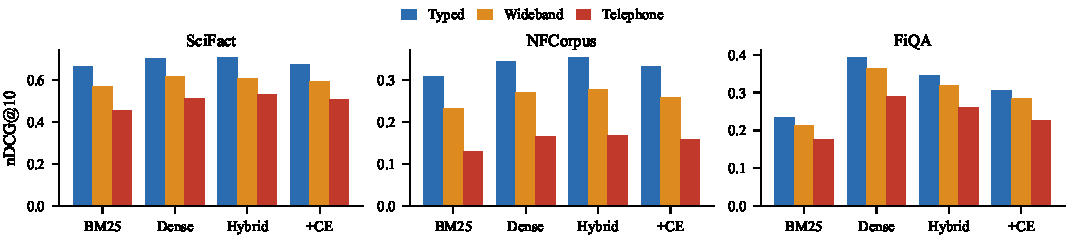
\includegraphics[width=\textwidth]{fig1_robustness.pdf}
\caption{nDCG@10 for typed and spoken queries. +CE: BM25 re-ranked by MiniLM.}
\label{fig:robust}
\end{figure*}

\begin{table}[t]
\caption{Relative nDCG@10 Change, Typed \ra{} Spoken (Wideband / Telephone, \%)}
\label{tab:relative}
\centering\footnotesize\setlength{\tabcolsep}{4pt}
\begin{tabular}{@{}lccc@{}}
\toprule
System & SciFact & NFCorpus & FiQA \\
\midrule
BM25 & $-14.7$ / $-31.4$ & $-24.7$ / $-58.1$ & $-8.0$ / $-24.8$ \\
Dense & $-12.2$ / $-26.9$ & $-21.2$ / $-51.9$ & $-7.1$ / $-25.8$ \\
Hybrid & $-13.6$ / $-24.5$ & $-21.2$ / $-52.5$ & $-7.3$ / $-24.1$ \\
BM25\ra CE & $-11.8$ / $-24.5$ & $-21.7$ / $-52.4$ & $-7.3$ / $-25.9$ \\
\bottomrule
\end{tabular}
\end{table}

\subsection{Noise-aware fine-tuning (RQ2)}
Fig.~\ref{fig:ft} and Table~\ref{tab:ft} summarise the fine-tuning study, macro-averaged over the three collections. Two findings hold across seeds and both protocols. First, fine-tuning on clean in-domain text makes the reranker more fragile: the typed-to-telephone drop widens from 31.9\% to 35.4\% (A) and 35.8\% (B). Second, training on transcripts recovers part of this loss: over the telephone, FT-noisy and FT-mixed beat FT-clean on all three collections, significantly on NFCorpus and FiQA under protocol~A and on all three under protocol~B (Table~\ref{tab:phone}). On typed queries they are not significantly different from FT-clean.

However, no labelled variant beats the zero-shot reranker on spoken queries. With about 1.2k training queries, fine-tuning significantly hurts NFCorpus for every labelled variant and leaves SciFact and FiQA close to zero-shot.

Consistency distillation behaves differently. FT-distill is the only variant that is never significantly worse than zero-shot in any collection, condition or protocol. It removes the NFCorpus damage (telephone nDCG@10 0.156 vs.\ 0.157 zero-shot and 0.120 for FT-clean), is significantly better than FT-clean on NFCorpus and FiQA in every condition, and is the best reranker on the macro average in all conditions (0.299 vs.\ 0.297 over the telephone). Its seed-to-seed standard deviation is at most 0.002, against up to 0.024 for labelled variants. Its gain over zero-shot is small and not significant.

\begin{figure}[t]
\centering
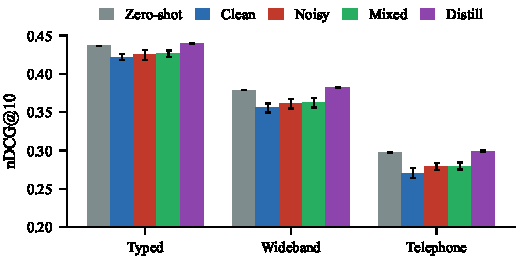
\includegraphics[width=\columnwidth]{fig2_finetuning.pdf}
\caption{MiniLM fine-tuning variants (macro nDCG@10, protocol B; bars: s.d.\ over three seeds).}
\label{fig:ft}
\end{figure}

\begin{table}[t]
\caption{Macro nDCG@10 Over Three Collections and Three Seeds}
\label{tab:ft}
\centering\footnotesize\setlength{\tabcolsep}{4pt}
\begin{tabular}{@{}llcccc@{}}
\toprule
Reranker & Prot. & Typed & Wide & Phone & Drop \\
\midrule
Zero-shot & -- & 0.436 & 0.379 & 0.297 & $-31.9\%$ \\
\midrule
FT-clean & A & 0.426 & 0.361 & 0.275 & $-35.4\%$ \\
FT-noisy & A & 0.433 & 0.371 & 0.288 & $-33.4\%$ \\
FT-mixed & A & 0.431 & 0.370 & 0.287 & $-33.4\%$ \\
FT-distill & A & \textbf{0.440} & \textbf{0.382} & \textbf{0.300} & $-31.9\%$ \\
\midrule
FT-clean & B & 0.422 & 0.355 & 0.271 & $-35.8\%$ \\
FT-noisy & B & 0.425 & 0.361 & 0.279 & $-34.3\%$ \\
FT-mixed & B & 0.426 & 0.362 & 0.280 & $-34.4\%$ \\
FT-distill & B & \textbf{0.440} & \textbf{0.382} & \textbf{0.299} & $-31.9\%$ \\
\bottomrule
\end{tabular}
\end{table}

\begin{table}[t]
\caption{Telephone Queries, Protocol B: nDCG@10 (Mean $\pm$ s.d.)}
\label{tab:phone}
\centering\footnotesize\setlength{\tabcolsep}{3pt}
\begin{tabular}{@{}lccc@{}}
\toprule
Reranker & SciFact & NFCorpus & FiQA \\
\midrule
Zero-shot & 0.509 & 0.157 & 0.226 \\
FT-clean & 0.487\phantom{$^{\ddagger}$}$\pm$.012 & 0.120$^{\dagger}$\phantom{$^{\ddagger}$}$\pm$.001 & 0.205$^{\dagger}$\phantom{$^{\ddagger}$}$\pm$.010 \\
FT-noisy & 0.504$^{\ddagger}$$\pm$.007 & 0.124$^{\dagger\ddagger}$$\pm$.003 & 0.210$^{\dagger\ddagger}$$\pm$.006 \\
FT-mixed & 0.503$^{\ddagger}$$\pm$.007 & 0.125$^{\dagger\ddagger}$$\pm$.004 & 0.211$^{\dagger\ddagger}$$\pm$.005 \\
FT-distill & 0.515\phantom{$^{\ddagger}$}$\pm$.002 & 0.156$^{\ddagger}$\phantom{$^{\dagger}$}$\pm$.000 & 0.227$^{\ddagger}$\phantom{$^{\dagger}$}$\pm$.000 \\
\bottomrule
\multicolumn{4}{@{}l}{$^{\dagger}p<0.05$ vs.\ zero-shot; $^{\ddagger}p<0.05$ vs.\ FT-clean.}
\end{tabular}
\end{table}

The held-out voice follows the same pattern. Over the telephone, FT-mixed (protocol~B) trails zero-shot by 0.016 nDCG@10 on the four training voices and by 0.021 on the unseen Irish voice, so the models do not simply memorise training voices.

\subsection{Effectiveness, latency and model size (RQ3)}
Fig.~\ref{fig:latency} relates re-ranking depth to effectiveness and latency (batch size equal to depth, warm model). At the production depth of 25, re-ranking takes about 1.1\,s (median) on a 4-thread CPU and about 80\,ms on a T4 GPU. Re-ranking 10 candidates costs about 0.4\,s on CPU and keeps roughly half or more of the depth-25 gain on every collection. A 12-layer cross-encoder (33.4M) improves SciFact significantly (0.687 vs.\ 0.674, $p=0.013$) but not NFCorpus or FiQA, and 512 instead of 256 input tokens changes nothing significantly.

\begin{figure*}[t]
\centering
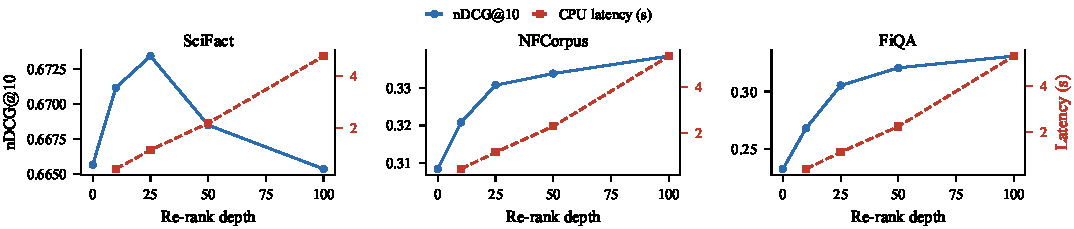
\includegraphics[width=\textwidth]{fig3_depth_latency.pdf}
\caption{Re-ranking depth vs.\ nDCG@10 and median CPU latency (depth 0 = BM25 only).}
\label{fig:latency}
\end{figure*}

\subsection{Real speech across English dialects (RQ4)}
On SD-QA, real speech lowers the production pipeline (BM25\ra CE) from 0.581 on typed questions by 11.2\% on average over the 21 conditions, from 3.3\% for US speakers to 21.9\% for South Indian speakers with the en-IN model, the worst condition. The four Indian-English conditions lose 16.9\% on average, comparable only to Kenyan and Nigerian speech with the en-US model (Fig.~\ref{fig:dialects}). As with synthetic speech, all pipelines lose similar proportions.

The ASR model matters as much as the dialect (Table~\ref{tab:asr}). A localised model significantly improves retrieval for five dialects, by up to 0.037 nDCG@10 (Australia). For both Indian dialects the opposite holds: the en-IN model is significantly worse than en-US ($-0.020$ North, $-0.026$ South), matching its higher WER on these recordings.

\begin{figure*}[t]
\centering
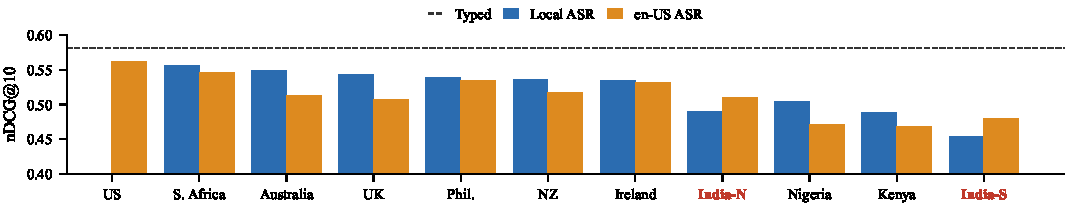
\includegraphics[width=\textwidth]{fig4_sdqa_dialects.pdf}
\caption{SD-QA: BM25\ra CE nDCG@10 per dialect with the local and the en-US ASR model. Indian dialects in red.}
\label{fig:dialects}
\end{figure*}

\begin{table}[t]
\caption{Local vs.\ en-US ASR on the Same Speakers (BM25\ra CE)}
\label{tab:asr}
\centering\footnotesize\setlength{\tabcolsep}{3.5pt}
\begin{tabular}{@{}llcccc@{}}
\toprule
Dialect & Model & WER loc./US & nDCG loc. & nDCG US & $\Delta$ \\
\midrule
UK & en-GB & .080 / .109 & 0.543 & 0.508 & $+0.035^{*}$ \\
Australia & en-AU & .082 / .102 & 0.549 & 0.513 & $+0.037^{*}$ \\
Nigeria & en-NG & .118 / .156 & 0.505 & 0.471 & $+0.034^{*}$ \\
Kenya & en-KE & .154 / .177 & 0.488 & 0.468 & $+0.021^{*}$ \\
N. Zealand & en-NZ & .067 / .089 & 0.536 & 0.518 & $+0.018^{*}$ \\
S. Africa & en-ZA & .069 / .078 & 0.556 & 0.546 & $+0.010$ \\
Ireland & en-IE & .083 / .086 & 0.535 & 0.532 & $+0.003$ \\
Philippines & en-PH & .084 / .076 & 0.538 & 0.535 & $+0.003$ \\
India-N & en-IN & .129 / .102 & 0.490 & 0.510 & $-0.020^{*}$ \\
India-S & en-IN & .176 / .120 & 0.454 & 0.479 & $-0.026^{*}$ \\
\bottomrule
\multicolumn{6}{@{}l}{$^{*}p<0.05$, paired randomization test.}
\end{tabular}
\end{table}

Table~\ref{tab:sdqa_ft} applies the BEIR-trained rerankers to SD-QA. The labelled variants stay within $\pm0.002$ of zero-shot in every group, so the fragility from clean fine-tuning on BEIR does not carry over to out-of-domain Wikipedia questions. FT-distill scores highest in every speech group, most clearly on Indian speech with the en-IN model (0.475 vs.\ 0.472), but the differences are small: uncorrected $p$ against zero-shot is 0.016--0.08, and none survives Holm correction.

\begin{table}[t]
\caption{BEIR-Trained Rerankers on SD-QA (nDCG@10, BM25 Top-25)}
\label{tab:sdqa_ft}
\centering\footnotesize\setlength{\tabcolsep}{2.6pt}
\begin{tabular}{@{}lcccccc@{}}
\toprule
Group & Zero & Clean & Noisy & Mixed & Distill & $p$\textsuperscript{a} \\
\midrule
Typed & .581 & .582 & .580 & .581 & \textbf{.586} & .030 \\
All speech (21) & .516 & .515 & .516 & .516 & \textbf{.519} & .079 \\
Indian (4) & .483 & .482 & .483 & .484 & \textbf{.486} & .029 \\
Indian, en-IN & .472 & .470 & .471 & .471 & \textbf{.475} & .016 \\
US & .562 & \textbf{.564} & \textbf{.564} & \textbf{.564} & \textbf{.564} & .279 \\
\bottomrule
\multicolumn{7}{@{}l}{\textsuperscript{a}Uncorrected, distill vs.\ zero-shot. Protocol B, mean of 3 seeds.}
\end{tabular}
\end{table}

The first stage, not the reranker, limits the production pipeline on SD-QA (Table~\ref{tab:first}, Fig.~\ref{fig:pipes}). On real speech BM25 retrieves only 80.5\% of relevant passages in its top 100, against 90.2\% for dense retrieval. Re-ranking a hybrid BM25\,+\,dense list instead of the BM25 list raises nDCG@10 from 0.516 to 0.607 on real speech (0.472 to 0.552 for Indian speech with en-IN) and is significantly better than dense retrieval alone ($p<0.001$). The hybrid pipeline also loses a smaller share to speech ($-9.5\%$ vs.\ $-11.2\%$). This comparison was not in the original analysis plan, so we report it as exploratory and test it confirmatorily in Section~\ref{sec:prereg}.

\begin{table}[t]
\caption{First-Stage Choice on SD-QA: nDCG@10 (Recall@100)}
\label{tab:first}
\centering\footnotesize\setlength{\tabcolsep}{2.4pt}
\begin{tabular}{@{}lccccc@{}}
\toprule
Group & BM25 & Dense & \cell{BM25\\\ra CE} & \cell{Hybrid\\\ra CE} & \cell{Hybrid\\\ra Distill} \\
\midrule
Typed & .375 (.897) & .615 (.987) & .581 & .671 & \textbf{.677} \\
Speech (21) & .323 (.805) & .537 (.902) & .516 & .607 & \textbf{.611} \\
Indian (4) & .304 (.771) & .505 (.866) & .483 & .572 & \textbf{.576} \\
Indian, en-IN & .294 (.752) & .478 (.839) & .472 & .552 & \textbf{.557} \\
\bottomrule
\end{tabular}
\end{table}

\begin{figure}[t]
\centering
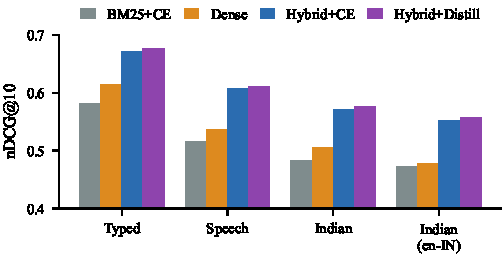
\includegraphics[width=\columnwidth]{fig5_sdqa_pipelines.pdf}
\caption{SD-QA: first-stage choice on typed and real spoken questions.}
\label{fig:pipes}
\end{figure}

\subsection{Pre-registered follow-up}
\label{sec:prereg}
Before further experiments we pre-registered six hypotheses (C1--C6), test sets and statistical tests, committed to the project repository before any result. All six were run as specified and are reported here, including the one that failed. The confirmatory test sets were new: SD-QA re-transcribed with Whisper base.en (704 questions $\times$ 11 dialects after dropping 43 questions with no Kenyan recording), HeySQuAD dev~\cite{heysquad} (1,002 human-spoken questions over 11,559 SQuAD paragraphs) and SLUE-SQA-5 test~\cite{slue} (2,382 real-speech questions over 3,192 documents).

\textbf{Modern reranker (C2).} We repeated the fine-tuning study with \texttt{bge-reranker-base}~\cite{bgem3} (278M, XLM-RoBERTa) using identical data and hyper-parameters (fp16, protocol B, three seeds). Both findings replicate and the distillation result strengthens (Table~\ref{tab:bge}, Fig.~\ref{fig:bge}). Clean fine-tuning widens the typed-to-telephone drop by 2.8 points (95\% CI 0.7--4.8) and, with noisy fine-tuning, significantly hurts NFCorpus and FiQA. Distillation is significantly better than zero-shot in 7 of 9 dataset--condition cells and never worse, raising macro telephone nDCG@10 from 0.282 to 0.295 (seed s.d.\ $\le0.001$). Zero-shot \texttt{bge-reranker-v2-m3} (568M) loses as large a share to telephone speech as the 22.7M MiniLM ($-32.3\%$ vs.\ $-31.9\%$), so model size alone does not protect against ASR errors.

\begin{table}[t]
\caption{bge-reranker-base on BEIR (Macro nDCG@10, Protocol B)}
\label{tab:bge}
\centering\footnotesize\setlength{\tabcolsep}{3pt}
\begin{tabular}{@{}lccccc@{}}
\toprule
Reranker & Typed & Wide & Phone & Drop & $\Delta$ drop [95\% CI] \\
\midrule
Zero-shot & 0.420 & 0.365 & 0.282 & $-32.9\%$ & -- \\
FT-clean & 0.421 & 0.362 & 0.271 & $-35.7\%$ & $-2.8$ [$-4.8$, $-0.7$] \\
FT-noisy & 0.413 & 0.357 & 0.271 & $-34.3\%$ & $-1.4$ [$-3.5$, $+0.6$] \\
FT-distill & \textbf{0.431} & \textbf{0.376} & \textbf{0.295} & $-31.5\%$ & $+1.4$ [$0.0$, $+2.7$] \\
\bottomrule
\end{tabular}
\end{table}

\begin{figure}[t]
\centering
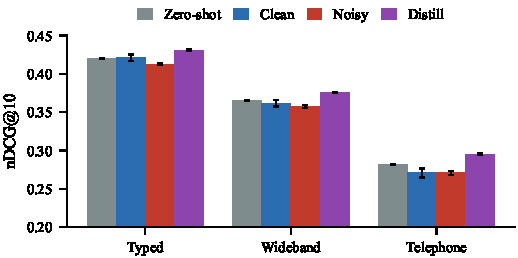
\includegraphics[width=\columnwidth]{fig6_bge_finetuning.pdf}
\caption{bge-reranker-base fine-tuning variants (macro nDCG@10; bars: s.d.\ over three seeds).}
\label{fig:bge}
\end{figure}

\textbf{Which words break (C4).} We aligned each question to its transcript and tagged its words with spaCy, then regressed the per-query change in nDCG@10 on the error rates of content words (nouns, proper nouns, numbers, adjectives, main verbs) and of function words. Content-word errors drive the loss (Table~\ref{tab:words}, Fig.~\ref{fig:words}): on SD-QA a fully misrecognised content vocabulary costs 0.65 nDCG@10, while function-word errors do no harm. A misrecognised named entity alone costs 0.27 on SD-QA. The difference between the coefficients is significant in every group (query-cluster bootstrap).

\textbf{Where the loss happens (C5).} Among spoken queries that lose effectiveness, the relevant passage is missing from the BM25 top 25 in 68\% of cases on SD-QA with Whisper (95\% CI 64--72\%), 53\% with Google ASR, 56\% on BEIR telephone (51--61\%) and 42\% on wideband BEIR, confirming the pre-registered prediction ($>50\%$ on SD-QA-Whisper and BEIR telephone). In these cases the reranker never sees the right passage.

\begin{table}[t]
\caption{Effect of Word Errors on nDCG@10 and Share of Losses Caused by First-Stage Recall Failure}
\label{tab:words}
\centering\scriptsize\setlength{\tabcolsep}{2.4pt}
\begin{tabular}{@{}lccc@{}}
\toprule
Group & $\beta$ content & $\beta$ function & Recall fail. \\
\midrule
SD-QA (Whisper) & $-.639$ [$-.716$, $-.569$] & $+.046$ [$-.016$, $+.111$] & 68\% [64, 72] \\
SD-QA (Google) & $-.646$ [$-.745$, $-.553$] & $+.117$ [$+.034$, $+.213$] & 53\% [47, 59] \\
BEIR wide & $-.369$ [$-.498$, $-.252$] & $-.025$ [$-.134$, $+.069$] & 42\% [35, 50] \\
BEIR phone & $-.363$ [$-.443$, $-.285$] & $-.011$ [$-.086$, $+.061$] & 56\% [51, 61] \\
\bottomrule
\multicolumn{4}{@{}l}{OLS coefficients with 95\% query-cluster bootstrap CIs.}
\end{tabular}
\end{table}

\begin{figure}[t]
\centering
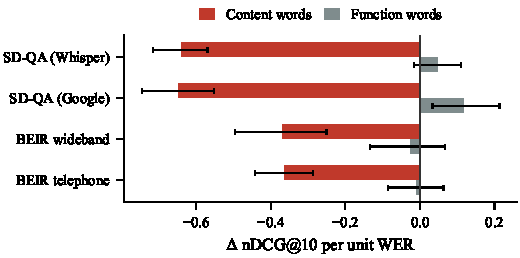
\includegraphics[width=\columnwidth]{fig7_word_errors.pdf}
\caption{Effect of content- and function-word errors on nDCG@10 (95\% CI).}
\label{fig:words}
\end{figure}

\textbf{First stage on new real speech (C1, confirmed).} Re-ranking a hybrid list beats re-ranking a BM25 list on all three new test sets, each significant after Holm correction (Table~\ref{tab:c1}, Fig.~\ref{fig:c1}): $+0.085$ nDCG@10 on SD-QA-Whisper, $+0.046$ on SLUE-SQA-5 and $+0.010$ on HeySQuAD, where BM25 alone already scores 0.85. The exploratory SD-QA finding therefore replicates on unseen data and a different recogniser.

\begin{table}[t]
\caption{C1: BM25 vs.\ Hybrid Candidates, Re-Ranked by MiniLM}
\label{tab:c1}
\centering\footnotesize\setlength{\tabcolsep}{2.6pt}
\begin{tabular}{@{}lrcccccc@{}}
\toprule
Test set & $n$ & BM25 & Dense & \cell{BM25\\\ra CE} & \cell{Hybrid\\\ra CE} & $\Delta$ & $p$\textsuperscript{a} \\
\midrule
SD-QA-Whisper & 704 & .286 & .489 & .469 & \textbf{.554} & $+.085$ & $<$.001 \\
HeySQuAD & 1,002 & .853 & .740 & .896 & \textbf{.906} & $+.010$ & .023 \\
SLUE-SQA-5 & 2,382 & .332 & .393 & .469 & \textbf{.515} & $+.046$ & $<$.001 \\
\bottomrule
\multicolumn{8}{@{}l}{\textsuperscript{a}Holm-corrected over three tests. nDCG@10 on spoken queries.}
\end{tabular}
\end{table}

\begin{figure}[t]
\centering
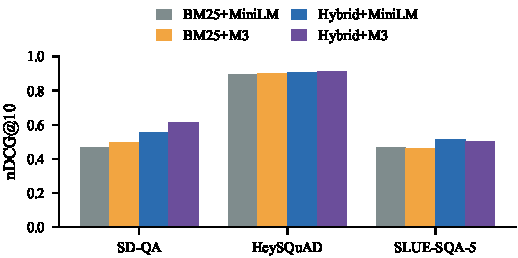
\includegraphics[width=\columnwidth]{fig9_first_stage.pdf}
\caption{First stage and reranker on the new real-speech test sets (M3: bge-reranker-v2-m3).}
\label{fig:c1}
\end{figure}

\textbf{Real vs.\ synthetic training noise (C3, not supported).} We predicted that training on real speech errors would transfer to real accented speech better than training on synthetic TTS errors. The opposite held (Table~\ref{tab:c3}, Fig.~\ref{fig:c3}). On the same 1,985 HeySQuAD questions, models trained on synthetic-speech transcripts were never worse than those trained on real-speech transcripts, and on SLUE-SQA-5 they were significantly better (FT-noisy 0.447 vs.\ 0.385; distillation 0.467 vs.\ 0.421; $p<0.001$). The real transcripts had twice the WER of the synthetic ones (0.150 vs.\ 0.075), so more of them no longer expressed the question; at this scale label noise, not realism, appears to dominate. Labelled fine-tuning again fell below zero-shot on every out-of-domain set.

\begin{table}[t]
\caption{C3: MiniLM Trained on 1,985 HeySQuAD Questions (nDCG@10)}
\label{tab:c3}
\centering\footnotesize\setlength{\tabcolsep}{2.4pt}
\begin{tabular}{@{}lcccccc@{}}
\toprule
& & & \multicolumn{2}{c}{FT-noisy} & \multicolumn{2}{c}{Distill} \\
\cmidrule(lr){4-5}\cmidrule(l){6-7}
Test set & Zero & Clean & Real & TTS & Real & TTS \\
\midrule
SD-QA-Whisper & .469 & .452 & .455 & .459 & .473 & \textbf{.475} \\
SD-QA, Indian & .448 & .434 & .436 & .441 & .451 & \textbf{.453} \\
SLUE-SQA-5 & \textbf{.469} & .450 & .385$^{\ddagger}$ & .447 & .421$^{\ddagger}$ & .467 \\
HeySQuAD\textsuperscript{a} & .896 & .906 & .904 & \textbf{.908} & .902 & .904 \\
\bottomrule
\multicolumn{7}{@{}l}{$^{\ddagger}$Worse than TTS counterpart, $p<0.001$ (Holm over 6 tests).}\\
\multicolumn{7}{@{}l}{\textsuperscript{a}In-domain. Mean of 3 seeds.}
\end{tabular}
\end{table}

\begin{figure*}[t]
\centering
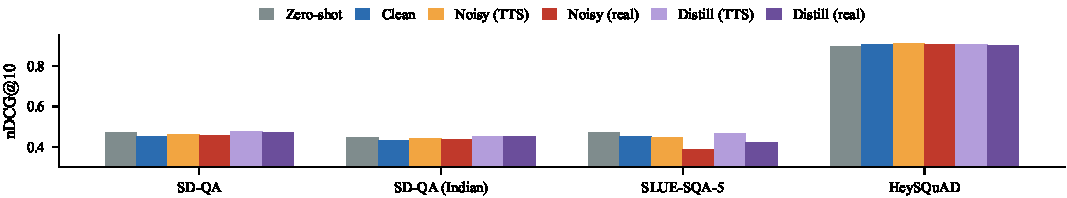
\includegraphics[width=\textwidth]{fig8_real_vs_synth.pdf}
\caption{Training on real vs.\ synthetic (TTS) speech errors: HeySQuAD-trained MiniLM.}
\label{fig:c3}
\end{figure*}

\textbf{Stronger distillation (C6, confirmed).} On validation only, we compared a 568M teacher (\texttt{bge-reranker-v2-m3}) with BM25 or hybrid candidates and temperatures 1, 2 and 4, plus the best of these trained on BEIR and HeySQuAD. The selected configuration (hybrid candidates, $\tau=4$, BEIR data) was retrained with three seeds and tested once. The 22.7M MiniLM student significantly beats its zero-shot self on all three pre-registered test groups (Table~\ref{tab:c6}), the first significant gain over zero-shot for the small model in this study.

\begin{table}[t]
\caption{C6: Distilled vs.\ Zero-Shot MiniLM (nDCG@10, 3 Seeds)}
\label{tab:c6}
\centering\footnotesize\setlength{\tabcolsep}{4pt}
\begin{tabular}{@{}lcccc@{}}
\toprule
Test set & Zero-shot & Distilled & $\Delta$ & $p$ (Holm) \\
\midrule
BEIR spoken\textsuperscript{a} & 0.313 & \textbf{0.321} & $+0.008$ & $<$0.001 \\
SD-QA-Whisper & 0.469 & \textbf{0.476} & $+0.007$ & 0.004 \\
SLUE-SQA-5 & 0.469 & \textbf{0.475} & $+0.006$ & 0.004 \\
\bottomrule
\multicolumn{5}{@{}l}{\textsuperscript{a}Three collections $\times$ two channels.}
\end{tabular}
\end{table}

\textbf{Stronger ASR (descriptive).} Re-transcribing SD-QA with Whisper large-v3-turbo instead of base.en more than halves the WER in every dialect (India-South 0.190 \ra{} 0.075) and recovers most of the loss: BM25\ra CE on India-South rises from 0.438 to 0.531, against 0.582 for typed questions. The Indian-English gap to US speakers narrows from 0.10 to about 0.03 nDCG@10.

\subsection{Repairing recall before the reranker (RQ5, pre-registered)}
Because more than half of the failures happen before the reranker (C5) and are caused by misrecognised content words (C4), a second study tested two training-free repairs that act on the transcript or the index. Its hypotheses and every setting were committed before any run.

\textbf{Listen Twice (LT).} Whisper base.en transcribes the call (pass~1). The transcript retrieves the hybrid top-5 passages. Their 30 rarest content words (Zipf frequency $<4$, ranked by passages containing the word $\times$ IDF) become Whisper's decoding prompt, and the same audio is transcribed again (pass~2) before the usual hybrid retrieval and re-ranking. Two controls isolate the mechanism: RND prompts with words from five random non-relevant passages, and ORC prompts with words from the relevant passage, an upper bound that no deployment can reach.

\textbf{Mishear the Corpus (MC).} Offline, up to 40,000 rare words of each corpus are spoken by two Piper TTS voices and transcribed by the same Whisper model. When the recogniser mishears a word (``conrad'' \ra{} ``comrade'', ``quebec'' \ra{} ``quiver''), the misheard tokens are added to the unused section field of every passage containing it. The production query builder is unchanged, and the reranker still reads the original passage. PH, a classic phonetic-indexing baseline~\cite{ng98}, fuses BM25 over Metaphone codes with word BM25.

\textbf{Results.} Table~\ref{tab:p4} gives the 12 pre-registered tests on Hybrid\ra CE nDCG@10 (Holm over all 12). LT significantly improves SD-QA ($+0.017$, $p_\text{Holm}=0.001$); on HeySQuAD and SLUE-SQA-5 it is directionally better but not significant. LT beats the random-prompt control on all three sets (H2), so the effect comes from the retrieved words, not from prompting: an unrelated prompt is neutral or harmful. MC gives no significant gain and does not beat phonetic indexing (H3, H4 not supported).

\begin{table}[t]
\caption{Part 4 Pre-Registered Tests (Hybrid\ra CE, nDCG@10)}
\label{tab:p4}
\centering\footnotesize\setlength{\tabcolsep}{3pt}
\begin{tabular}{@{}llcccc@{}}
\toprule
Test & Set & A & B & $\Delta$ [95\% CI] & $p_\text{Holm}$ \\
\midrule
\multirow{3}{*}{H1: LT $>$ pass 1} & SD-QA & \textbf{.571} & .554 & $+.017$ [$+.012$, $+.023$] & \textbf{.001} \\
 & HeySQuAD & .912 & .906 & $+.006$ [$-.000$, $+.013$] & .619 \\
 & SLUE & .518 & .515 & $+.003$ [$-.002$, $+.008$] & 1.00 \\
\midrule
\multirow{3}{*}{H2: LT $>$ RND} & SD-QA & \textbf{.571} & .554 & $+.017$ [$+.011$, $+.023$] & \textbf{.001} \\
 & HeySQuAD & \textbf{.912} & .899 & $+.013$ [$+.006$, $+.021$] & \textbf{.003} \\
 & SLUE & \textbf{.518} & .509 & $+.008$ [$+.003$, $+.014$] & \textbf{.008} \\
\midrule
\multirow{3}{*}{H3: MC $>$ pass 1} & SD-QA & .555 & .554 & $+.001$ [$-.002$, $+.004$] & 1.00 \\
 & HeySQuAD & .907 & .906 & $+.001$ [$-.001$, $+.004$] & 1.00 \\
 & SLUE & .516 & .515 & $+.001$ [$-.002$, $+.004$] & 1.00 \\
\midrule
\multirow{3}{*}{H4: MC $>$ PH} & SD-QA & .555 & .558 & $-.003$ [$-.008$, $+.002$] & 1.00 \\
 & HeySQuAD & .907 & .906 & $+.001$ [$-.003$, $+.004$] & 1.00 \\
 & SLUE & .516 & .515 & $+.000$ [$-.003$, $+.004$] & 1.00 \\
\bottomrule
\multicolumn{6}{@{}l}{SD-QA: per-question mean over 11 dialects (704 questions).}
\end{tabular}
\end{table}

\begin{table}[t]
\caption{Part 4 Systems: nDCG@10 (CE, M3) and Hybrid Recall@25}
\label{tab:p4sys}
\centering\footnotesize\setlength{\tabcolsep}{2.6pt}
\begin{tabular}{@{}lccccccc@{}}
\toprule
& \multicolumn{3}{c}{SD-QA} & \multicolumn{2}{c}{HeySQuAD} & \multicolumn{2}{c}{SLUE} \\
\cmidrule(lr){2-4}\cmidrule(lr){5-6}\cmidrule(l){7-8}
System & CE & M3 & R@25 & CE & M3 & CE & M3 \\
\midrule
Typed (reference) & .669 & .748 & .900 & .938 & .951 & .563 & .532 \\
\midrule
Pass 1 (baseline) & .554 & .613 & .767 & .906 & .915 & .515 & .501 \\
Phonetic index (PH) & .558 & -- & .776 & .906 & -- & .515 & -- \\
Mishear the Corpus & .555 & .613 & .767 & .907 & .917 & .516 & .501 \\
Random prompt (RND) & .554 & -- & .768 & .899 & -- & .509 & -- \\
Listen Twice (LT) & .571 & .635 & .787 & .912 & .923 & .518 & .497 \\
LT + MC & \textbf{.576} & \textbf{.637} & .791 & \textbf{.914} & \textbf{.925} & .518 & .497 \\
LT-fuse (pass 1 + 2) & .573 & -- & \textbf{.792} & .909 & -- & \textbf{.520} & -- \\
\midrule
Oracle prompt (bound) & .630 & -- & .855 & .930 & -- & .538 & -- \\
\bottomrule
\end{tabular}
\end{table}

\begin{figure*}[t]
\centering
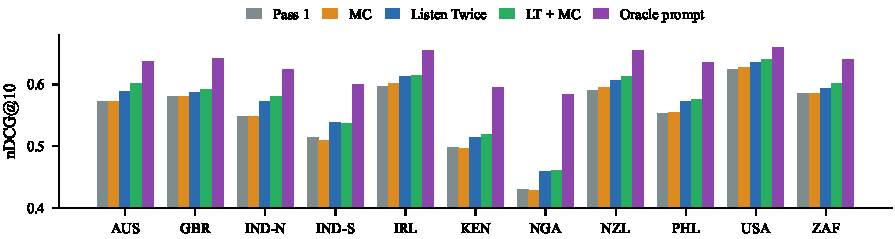
\includegraphics[width=\textwidth]{fig10_listen_twice.pdf}
\caption{Part 4 on SD-QA by dialect (Hybrid\ra CE). Listen Twice gains most where pass 1 is worst (Nigerian, Indian English); the oracle prompt marks the remaining headroom.}
\label{fig:p4}
\end{figure*}

\textbf{Why LT works.} LT lowers the rare-word error rate from 0.378 to 0.262 on SD-QA (0.203 \ra{} 0.151 on HeySQuAD) and the WER from 0.156 to 0.141, and it raises hybrid Recall@25 from 0.767 to 0.787. Only 0.8--2.0\% of pass-2 transcripts contain a prompt word that was spoken in neither the question nor pass~1, so injection of unspoken words is rare. The gain is largest where recognition is worst (Fig.~\ref{fig:p4}): Nigerian $+0.030$, Indian-North $+0.024$, Indian-South $+0.026$, against $+0.011$ for US speakers. It replicates with the 568M bge-reranker-v2-m3 on SD-QA (0.613 \ra{} 0.635) and HeySQuAD (0.915 \ra{} 0.923). The pass-2 decode adds about 50\,ms per query on a T4 GPU, and re-decoding without a prompt reproduced pass~1 exactly (100\%).

\textbf{Confirmation bias.} A wrong first retrieval could lock in wrong words. On SD-QA, LT helps both when the pass-1 top-5 contained a relevant passage ($+0.019$, 525 questions) and when it did not ($+0.012$, 179). On HeySQuAD and SLUE the gain comes from questions that pass~1 had missed ($+0.066$ and $+0.012$), with small losses where pass~1 had already succeeded ($-0.001$, $-0.004$). LT-fuse, which fuses the pass-1 and pass-2 runs, removes most of these losses and gives the best SLUE score and SD-QA recall.

\textbf{Why MC does not.} The recogniser mishears 61--68\% of isolated rare words, and the expansion grows the index by 11--13\% of its tokens, yet ranking hardly changes. A word spoken in isolation by TTS is misheard differently from the same word inside a real accented question (``vietnamese'' \ra{} ``attendees''), so the indexed mishearings seldom match those in real transcripts. MC is harmless: it is non-inferior on typed queries for all three sets (margin $-0.005$), and adding it to LT gives the best SD-QA score (LT+MC $-$ LT $= +0.005$, $p=0.006$, secondary analysis). The oracle prompt still lies 0.05 nDCG@10 above LT on SD-QA, so better selection of bias words has headroom.

\section{Discussion}
\textbf{Why the reranker does not help on speech.} A cross-encoder reads query and passage together but cannot restore what the transcript has lost. When ASR replaces a key term with another real word, both the first stage and the reranker match the wrong term, so all pipelines lose a similar proportion.

\textbf{Why clean fine-tuning increases fragility.} Fine-tuning on clean in-domain queries appears to strengthen reliance on exact domain terminology, which is exactly what ASR corrupts. Exposure to transcripts counteracts this, in line with typo-aware training for text noise~\cite{zhuang21}.

\textbf{Why fine-tuning hurts NFCorpus.} NFCorpus has many relevant documents per query and incomplete judgments, so BM25 hard negatives likely include unjudged relevant documents, teaching the model to reject relevant passages. Distillation supports this indirectly: it uses the same queries and candidates but no labels, and removes the NFCorpus damage on both model families.

\textbf{Why distillation is safe but small.} Distillation anchors the student to the original model's ranking of each candidate list, which explains both its stability across seeds and its small effect. It helps when the transcript still contains the key terms, but not when ASR has removed them.

\textbf{Real speech and Indian English.} Real speech is milder than our telephone channel but still costs every pipeline about a tenth of its effectiveness, and Indian-English speakers lose the most, in line with known ASR weaknesses on Indian accents~\cite{svarah}. Because the en-IN recogniser made more errors on Indian speech than en-US, a deployment should choose its ASR model by measured accuracy on its own callers, not by locale name.

\textbf{Where the loss happens.} A reranker can only reorder what the first stage returns, so improving the candidate list helps far more than any change to the reranker, consistent with SQuTR's finding that the retrieval backend matters most~\cite{squtr}.

\textbf{The knowledge base can help the recogniser.} Listen Twice turns the retrieval system into context for ASR: a voice agent already holds the vocabulary its callers are likely to say, and passing it back to the recogniser repairs the content words that C4 identified. Because the prompt comes from the first retrieval, the method improves most when ASR is poor but not hopeless, which is the regime of accented callers. Simulating mishearings offline (MC) did not work, which suggests that ASR errors depend on context and voice more than on the word alone.

\textbf{Implications for voice agents.} (1) Speech quality, not the reranker, is the main lever; a cheap second ASR pass guided by the knowledge base (Listen Twice) is a practical way to raise it. (2) Re-rank a hybrid BM25\,+\,dense list rather than a BM25 list. (3) When adapting a reranker, prefer label-free consistency distillation, or at least include transcripts; clean fine-tuning makes it more fragile. (4) Choose the ASR model by measured accuracy for the target callers, especially for Indian English. (5) On CPU, reduce the re-ranking depth to fit a live turn or move the reranker to a GPU.

\section{Limitations}
The BEIR training speech is synthetic, and the SD-QA, HeySQuAD and SLUE recordings are not telephone audio; our telephone channel is simulated and lacks real codec artefacts and packet loss. We fine-tune two reranker families. Distillation gains on MiniLM are small in absolute terms ($+0.006$ to $+0.008$ nDCG@10) although significant on all pre-registered test sets. The training sets are small (1,184 BEIR and 1,985 HeySQuAD queries), hard negatives may include unjudged relevant documents, and the real HeySQuAD transcripts are noisier than the synthetic ones, so C3 compares noise levels as well as noise types. Latency was measured on Kaggle hardware, not on the deployment machine. Listen Twice was tested with one recogniser (Whisper base.en) and fixed settings ($K=5$, 30 words); its gain on HeySQuAD and SLUE-SQA-5 was not significant, and MC used isolated-word TTS, which does not reproduce the co-articulation and accents of real callers.

\section{Conclusion and Future Work}
Spoken queries reduce retrieval effectiveness by 7--25\% over wideband audio, 24--58\% over a telephone channel and 11--19\% on real speech, with Indian English among the hardest hit, and a cross-encoder reranker does not reduce this relative loss. Misrecognised content words drive the loss, and in more than half of the failures the relevant passage never reaches the reranker. Fine-tuning the reranker on clean text makes it more fragile to speech on two model families; label-free consistency distillation avoids this and, with a stronger teacher, significantly improves on the zero-shot reranker on every pre-registered test set. The largest gains come from outside the reranker: a hybrid first stage, confirmed on three new real-speech test sets, and a stronger recogniser. A training-free second ASR pass prompted with words from the first retrieval (Listen Twice) significantly improves real dialectal speech and helps most for the speakers hurt most, while indexing simulated mishearings does not. Future work will combine Listen Twice with stronger recognisers and better bias-word selection, simulate mishearings in sentence context rather than in isolation, re-rank ASR N-best lists, train on larger real-speech data filtered by WER, record real Indian-English telephone queries, and deploy the hybrid first stage with a distilled reranker in the voice agent.

\begin{thebibliography}{00}
\bibitem{zhuang22} S. Zhuang and G. Zuccon, ``CharacterBERT and self-teaching for improving the robustness of dense retrievers on queries with typos,'' in \textit{Proc. SIGIR}, 2022.
\bibitem{sdqa} F. Faisal, S. Keshava, M. M. I. Alam, and A. Anastasopoulos, ``SD-QA: Spoken dialectal question answering for the real world,'' in \textit{Findings of EMNLP}, 2021.
\bibitem{spokensquad} C.-H. Lee \textit{et al.}, ``Spoken SQuAD: A study of mitigating the impact of speech recognition errors on listening comprehension,'' in \textit{Proc. Interspeech}, 2018.
\bibitem{sidiropoulos} G. Sidiropoulos, S. Vakulenko, and E. Kanoulas, ``On the impact of speech recognition errors in passage retrieval for spoken question answering,'' in \textit{Proc. CIKM}, 2022, doi: 10.1145/3511808.3557662.
\bibitem{squtr} Y. Li \textit{et al.}, ``SQuTR: A robustness benchmark for spoken query to text retrieval under acoustic noise,'' arXiv:2602.12783, 2026.
\bibitem{bao} Z. Bao, ``Better retrieval, worse robustness: How multi-hop RAG amplifies upstream ASR errors,'' in \textit{Proc. EMNLP}, 2026, arXiv:2608.22872.
\bibitem{moriya} Y. Moriya and G. J. F. Jones, ``Improving noise robustness for spoken content retrieval using semi-supervised ASR and N-best transcripts for BERT-based ranking models,'' in \textit{Proc. IEEE SLT}, 2022, arXiv:2301.06056.
\bibitem{zhuang21} S. Zhuang and G. Zuccon, ``Dealing with typos for BERT-based passage retrieval and ranking,'' in \textit{Proc. EMNLP}, 2021, pp. 2836--2842.
\bibitem{ma} X. Ma, C. dos Santos, and A. O. Arnold, ``Contrastive fine-tuning improves robustness for neural rankers,'' in \textit{Findings of ACL-IJCNLP}, 2021, pp. 570--582.
\bibitem{penha} G. Penha, A. C\^{a}mara, and C. Hauff, ``Evaluating the robustness of retrieval pipelines with query variation generators,'' in \textit{Proc. ECIR}, 2022, pp. 397--412.
\bibitem{hagen} T. Hagen, H. Scells, and M. Potthast, ``Revisiting query variation robustness of transformer models,'' in \textit{Findings of EMNLP}, 2024.
\bibitem{nogueira} R. Nogueira and K. Cho, ``Passage re-ranking with BERT,'' arXiv:1901.04085, 2019.
\bibitem{beir} N. Thakur, N. Reimers, A. R\"{u}ckl\'{e}, A. Srivastava, and I. Gurevych, ``BEIR: A heterogeneous benchmark for zero-shot evaluation of information retrieval models,'' in \textit{Proc. NeurIPS Datasets and Benchmarks Track}, 2021.
\bibitem{rosa} G. M. Rosa \textit{et al.}, ``In defense of cross-encoders for zero-shot retrieval,'' arXiv:2212.06121, 2022.
\bibitem{minilm} W. Wang \textit{et al.}, ``MiniLM: Deep self-attention distillation for task-agnostic compression of pre-trained transformers,'' in \textit{Proc. NeurIPS}, 2020.
\bibitem{bge} S. Xiao \textit{et al.}, ``C-Pack: Packaged resources to advance general Chinese embedding,'' arXiv:2309.07597, 2023.
\bibitem{rrf} G. V. Cormack, C. L. A. Clarke, and S. B\"{u}ttcher, ``Reciprocal rank fusion outperforms Condorcet and individual rank learning methods,'' in \textit{Proc. SIGIR}, 2009.
\bibitem{whisper} A. Radford \textit{et al.}, ``Robust speech recognition via large-scale weak supervision,'' in \textit{Proc. ICML}, 2023.
\bibitem{koenecke} A. Koenecke \textit{et al.}, ``Careless Whisper: Speech-to-text hallucination harms,'' in \textit{Proc. ACM FAccT}, 2024.
\bibitem{adamw} I. Loshchilov and F. Hutter, ``Decoupled weight decay regularization,'' in \textit{Proc. ICLR}, 2019.
\bibitem{smucker} M. D. Smucker, J. Allan, and B. Carterette, ``A comparison of statistical significance tests for information retrieval evaluation,'' in \textit{Proc. CIKM}, 2007.
\bibitem{holm} S. Holm, ``A simple sequentially rejective multiple test procedure,'' \textit{Scand. J. Statist.}, vol. 6, no. 2, pp. 65--70, 1979.
\bibitem{heysquad} Y. Wu \textit{et al.}, ``HeySQuAD: A spoken question answering dataset,'' arXiv:2304.13689, 2023.
\bibitem{slue} S. Shon \textit{et al.}, ``SLUE Phase-2: A benchmark suite of diverse spoken language understanding tasks,'' in \textit{Proc. ACL}, 2023.
\bibitem{bgem3} J. Chen \textit{et al.}, ``BGE M3-Embedding: Multi-lingual, multi-functionality, multi-granularity text embeddings through self-knowledge distillation,'' arXiv:2402.03216, 2024.
\bibitem{peng23} P. Peng, B. Yan, S. Watanabe, and D. Harwath, ``Prompting the hidden talent of web-scale speech models for zero-shot task generalization,'' in \textit{Proc. Interspeech}, 2023.
\bibitem{ng98} K. Ng and V. W. Zue, ``Phonetic recognition for spoken document retrieval,'' in \textit{Proc. IEEE ICASSP}, 1998.
\bibitem{lee15} L.-S. Lee, J. Glass, H.-Y. Lee, and C.-A. Chan, ``Spoken content retrieval---Beyond cascading speech recognition with text retrieval,'' \textit{IEEE/ACM Trans. Audio, Speech, Lang. Process.}, vol. 23, no. 9, pp. 1389--1420, 2015.
\bibitem{svarah} T. Javed \textit{et al.}, ``Svarah: Evaluating English ASR systems on Indian accents,'' in \textit{Proc. Interspeech}, 2023.
\end{thebibliography}

\end{document}
